\chapter[Características Fractales del Pan]{Validación de los métodos: Características Fractales y Multifractales del Pan}

\section{Introducción}


Las imágenes generadas utilizando los métodos de los capítulos previos producen, en los seres humanos, la percepción de determinados materiales.
Lamentablemente, este fenómeno es difícilmente cuantizable.
La computación gráfica ha apelado históricamente a métodos subjetivos de validación de resultados, debido a la complejidad de los fenómenos involucrados.
Uno de ellos consiste en realizar pruebas con personas, entreg\'andoles im\'agenes verdaderas y sint\'eticas, sin que ellas sepan a cu\'al categor\'ia pertenece cada una, pidi\'endoles que clasifiquen las im\'agenes en verdaderas y sint\'eticas.
Si las im\'agenes sint\'eticas resultan ser clasificadas en un porcentaje adecuado como reales, se puede considerar al experimento como satisfactorio.
Si bien este método puede resultar interesante, se siguen requiriendo métodos automáticos y objetivos, ya que en este caso se sigue dependiendo de observadores subjetivos para evaluar la calidad de las imágenes.




Existen diversos criterios para evaluar la fidelidad de las im\'agenes resultantes.
Apelando a métodos matemáticos, podemos comparar imágenes por medio de extracci\'on de caracter\'isticas.
En el presente capítulo se comparan dimensiones fractales (DF) y multifractales de determinadas caracter\'isticas de muestras reales y sint\'eticas.


Gracias a estas t\'ecnicas, podemos validar los resultados obtenidos en los cap\'itulos anteriores con una base matem\'atica s\'olida, m\'as all\'a de la validaci\'on visual realizada por las personas, la cual es utilizada tradicionalmente en computaci\'on gr\'afica.
Además, las características fractales y multifractales capturan detalles esenciales que pueden ser utilizados para la clasificación de las muestras, superando a otros clasificadores del estado del arte.


\section{Dimensiones fractales de imágenes de pan}

Uno de los factores más importantes en la evaluación de la calidad de una muestra de pan es la estructura de su miga.
La observación de las burbujas, de distintos cortes de pan, nos revela una variación considerable en los tamaños y posiciones de las mismas, incluso si los cortes pertenecen a una única muestra de un tipo de pan.
Si bien estas estructuras parecen carecer de patrones que caractericen al material, en este capítulo mostraremos que es posible, a nivel estadístico, caracterizar sus distribuciones.

En \cite{Gonzales2008} se present\'o un trabajo de c\'alculo de distintas DFs sobre muestras de pan.
Las mismas son obtenidas a trav\'es de diversos algoritmos, diferentes a los utilizados en este trabajo.
Debido a esto, en esta sección utilizaremos dos métodos, con el objetivo de demostrar que una única dimensión fractal, si bien constituye una aproximación adecuada en muchos casos, no es lo suficientemente descriptiva para capturar la riqueza de las distribuciones de burbujas en distintos tipos de panes.
Esto será demostrado realizando una caracterización y clasificación de distintas imágenes de muestras de pan. 

Se utilizan las DFs de Korcak \cite{Mandelbrot1983} y la dimensi\'on Box \cite{Peitgen2004} sobre imágenes obtenidas por medios tradicionales (cámaras y escáneres), buscando caracterizar su estructura.


\subsection{Dimensi\'on Box}
La misma intenta simplificar el c\'alculo de la DF de Hausdorff, debido a que \'esta resulta muy dif\'icil de obtener \cite{Peitgen2004} (o imposible si el objeto no es estrictamente autosimilar).

Dada una imagen, se la subdividide en una grilla $M\times M$ donde el largo del lado de cada cuadrado formado es $\delta$. Si $N(\delta)$ representa el n\'umero de cuadrados que contienen al menos un p\'ixel resultado de una binarizaci\'on de la imagen (p\'ixel blanco) para ese $\delta$, la dimensi\'on Box $D_{b}$ queda definida como:\\

$D_{b} = \displaystyle\lim_{\delta \to 0}{\frac{\log(N(\delta))}{\log (1/\delta)}}$\\

En el algoritmo resultante se utiliza una imagen binarizada de la original. A partir de ella se seleccionan distintos $\delta$, realizando un conteo de cuadrados que contienen p\'ixeles blancos en cada caso (para evitar inestabilidad num\'erica, se utiliza un promedio de casos, estableciendo distintas posiciones de la grilla sobre la imagen). Finalmente se realiza un ajuste por regresi\'on lineal de los datos obtenidos en el espacio $\log-\log$, cuya pendiente es por definici\'on la DF Box de la imagen.

\subsection{Dimensi\'on Fractal de Korcak}
Esta DF fue introducida en \cite{Mandelbrot1983}, basada en un trabajo previo del cient\'ifico checo Kor$\check{c}$\'ak. La misma funciona como un descriptor de fragmentaci\'on de objetos en dos dimensiones. Su definici\'on formal es la siguiente \cite{Imre11}:

$N(A > a) = k a^{-K},$

\noindent
donde K es el exponente Korcak de fragmentaci\'on (patchiness), N es el n\'umero de fragmentos cuyo \'area $A$ es mayor que el valor $a$, y $k$ es una constante. La DF de Korcak, $D_{k}$, queda definida de la siguiente manera:

$K = D_{k}/2.$

El procedimiento para calcular $D_{k}$ consiste en ajustar una recta a partir de pares $(\log(a),\log(N))$. Consideramos a esta dimensión apropiada dado que las muestras de pan est\'an compuestas por burbujas de distinto tama\~no, resultantes del proceso de fabricación del mismo, por lo tanto, se busca que las muestras sint\'eticas posean caracter\'isticas similares de {\em fragmentaci\'on}.

\subsection{Segmentaci\'on de las Im\'agenes}
La imagen original es binarizada utilizando el algoritmo de Otsu \cite{Otsu79} para definir un valor de umbral, a partir del cual se decide si el p\'ixel ser\'a negro o blanco en la binarizaci\'on. 

%Un error muy com\'un utilizando este m\'etodo es que muchas regiones de la imagen donde el ojo detecta masa, son consideradas burbujas (color blanco). En estos casos se obtuvo un mejor resultado al definir un umbral $t$ para una imagen determinada (observando el resultado para cada imagen). La misma es transformada a escala de grises y se establece como burbuja a cualquier valor menor a $t$. En casos donde este procedimiento no resulta satisfactorio, se elige una subregi\'on de la imagen donde el algoritmo de segmentaci\'on presenta buenos resultados.

Si bien este algoritmo se utiliza de manera estándar en diversas aplicaciones, en el caso de fotografías o imágenes escaneadas de pan pueden existir variaciones en la iluminación dentro de la imagen.
Por esto, se presenta un algoritmo de umbralamiento local que obtiene binarizaciones más adecuadas para estas imágenes. 


\subsubsection{Binarización de migas de pan utilizando umbralamiento local}
Las binarizaciones se llevaron a cabo utilizando el algoritmo de umbralamiento local descripto en \cite{White83}. El mismo presentó mejores resultados que la utilización del algoritmo presentado en \cite{Huang95} y utilizado en \cite{Gonzales2008}, el cual utiliza un umbralamiento global de la imagen. Esto se debe a que sutiles variaciones en la iluminación de la misma muestra resultados incorrectos en la determinación de burbujas. En la Figura~\ref{fig:bread} se observa una imagen de cada tipo de pan (primera fila) y su binarización correspondiente utilizando el algoritmo descripto (segunda fila). Elementos pequeños de la imagen de $1$ o $2$ píxeles fueron removidos utilizando una operación de {\em opening} (erosión y dilatación) con un elemento estructurante de $2\times 2$. Este método presenta buenos resultados incluso con condiciones de iluminación variando sobre la imagen.

En cada píxel, el resultado de la binarización se computa a través de un promedio de los niveles de gris en una ventana que rodea ese píxel. Este promedio se compara con un umbral definido por el nivel de gris del píxel actual multiplicado por un número de bias y en caso de ser mayor, el píxel resultará blanco (en otro caso, negro), es decir:
\begin{equation}
\frac{\sum_{x,y \in W} f(x,y) }{W_{size}} \geq f(x_{c},y_{c}) \times bias,
\label{eqn:white}
\end{equation}
donde $x_{c},y_{c}$ son las coordenadas del píxel actual y  $W$ es la ventana que rodea al píxel. Los dos parámetros que definen al algoritmo son: el tamaño de la ventana ($W_{size}$) y el $bias$. 

Experimentalmente encontramos que estos parámetros dependen del método de captura utilizado. Los mejores valores para las muestras de escáner fueron $80$ para el tamaño de la ventana y $1.15 $ para el bias. En el caso de las muestras tomadas con una cámara digital, los valores óptimos fueron $80$ para la ventana y $1$ para el bias.  Estas diferencias parecen ser causadas por las diferentes condiciones de iluminación presentes en las imágenes. Queda planteado como trabajo a futuro la determinación automática de estos parámetros.


En la Fig.~\ref{bin} puede observarse una imagen y su binarizaci\'on.
La Fig.~\ref{fitbox} muestra los valores obtenidos en el c\'alculo de la dimensi\'on Box para esta imagen y la recta que ajusta estos valores. 
En la Fig.~\ref{fit} se observan los valores obtenidos por el algoritmo de Korcak para esta imagen y las rectas aproximantes (en la siguiente secci\'on se explica el por qu\'e de dos rectas aproximantes).

\begin{figure}
\centering
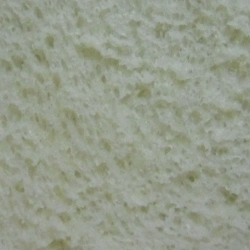
\includegraphics[width=5cm]{figures/lactal}
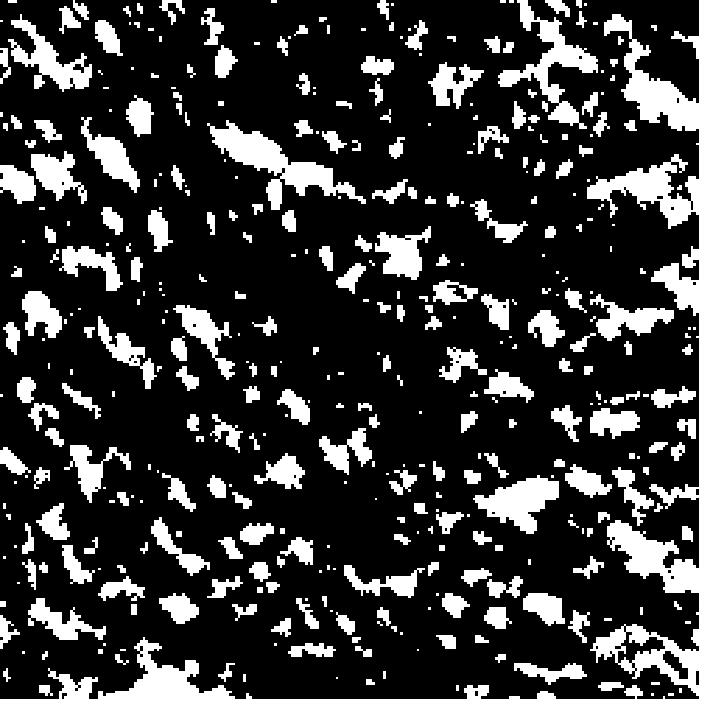
\includegraphics[width=5cm]{figures/lactalBin}
\caption{Imagen y su binarizaci\'on}
\label{bin}
\end{figure}



\begin{figure}
\centering
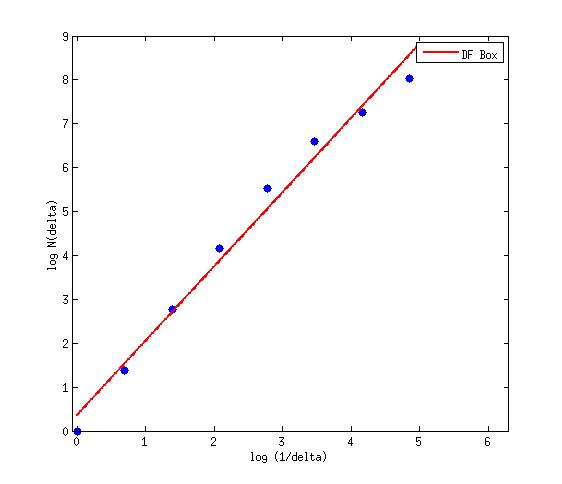
\includegraphics[width=8cm]{figures/fitbox}
\caption{Dimensi\'on Box de la imagen de la Figura \ref{bin}}
\label{fitbox}
\end{figure}


\begin{figure}
\centering
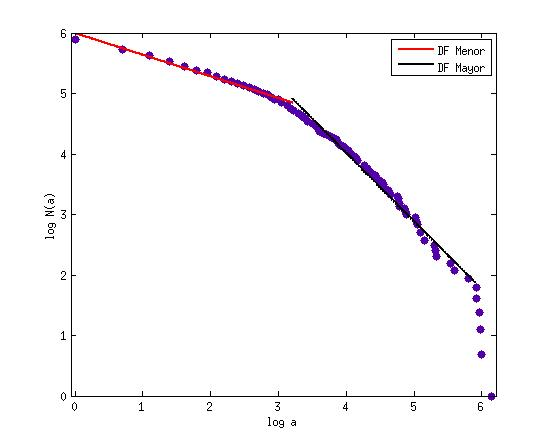
\includegraphics[width=8cm]{figures/lactal1PlotKorcak}
\caption{DFs de Korcak de la imagen de la Figura \ref{bin}}
\label{fit}
\end{figure}

\subsection{Dimensiones Estimadas}

En los diagramas $\log-\log $ obtenidos por el algoritmo (Korcak), puede observarse que una \'unica recta no ajusta correctamente los valores. Esto sugiere que las muestras presentan caracter\'isticas {\em multifractales} \cite{Mandelbrot1989}. Es decir que es posible calcular m\'as de una DF para la misma imagen. Se realizaron pruebas con pan lactal y mignon. Las DFs encontradas se incluyen en la Tabla \ref{tab:korcak}.

\begin{table}
\center
\begin{tabular}{|| l | l | l ||}
    \hline
     & DF (menor) & DF (mayor) \\    
    \hline
    Lactal 1 & 0.7152 & 2.214 \\
    \hline
    Lactal 2 & 0.8638 & 2.182 \\
    \hline
    Lactal 3 & 0.7598 & 2.046 \\
    \hline
    Lactal 4 & 0.8656 & 2.598 \\
    \hline
    Mignon 1 & 0.5068 & 1.1452\\
    \hline
    Mignon 2 & 0.4214 & 1.1608\\
    \hline
\end{tabular}
\caption{DFs de Korcak estimadas en muestras reales de pan}
\label{tab:korcak}
\end{table}

%Puede observarse que para distintos tipos de panes las DFs resultantes var\'ian de manera considerable, por lo cual es posible pensar a estas DF como clasificadores de muestras.

Para la regresi\'on por DF Box, los valores que se obtuvieron se muestran en la Tabla \ref{tab:box}.
Se observa cierta similitud entre los valores obtenidos, por lo cual resulta un par\'ametro \'util el cual deben cumplir las im\'agenes sint\'eticas.
%Sin embargo no resulta un par\'ametro adecuado para realizar clasificaci\'on de muestras.

\begin{table}
\begin{center}
\begin{tabular}{|| l | l | l ||}
    \hline
     & DF \\    
    \hline
    Lactal 1 & 1.692 \\
    \hline
    Lactal 2 & 1.761 \\
    \hline
    Lactal 3 & 1.743\\
    \hline
    Lactal 4 & 1.73 \\
    \hline
    Mignon 1 & 1.686 \\
    \hline
    Mignon 2 & 1.726 \\
    \hline
\end{tabular}
\caption{DFs Box estimadas en muestras reales de pan}
\label{tab:box}
\end{center}
\end{table}

\section[Características Multifractales del pan]{Caracterización y Clasificación de Imágenes de Pan Utilizando Características Fractales y Multifractales.}

La sección anterior demostró que cuando se intenta computar una DF para una imagen de pan, es difícil utilizar una única recta que ajuste adecuadamente los datos obtenidos.
La utilización de más de una recta de ajuste permite reducir los errores de las regresiones lineales.
Es decir, dentro de la imagen se presenta más de una DF.
Esto implica que necesitamos más de una DF para caracterizar adecuadamente una muestra.
En otras palabras, la teoría multifractal podría arrojar resultados más precisos sobre la composición de burbujas en la miga del pan.

El análisis fractal y multifractal ha probado ser útil para capturar propiedades útiles del material a representar.
Estas características han sido aplicadas con éxito en diferentes áreas, como medicina \cite{Andjelkovic2008,Yu2011} y clasificación de texturas \cite{Wendt2009}.
En el tópico de alimentos, estas técnicas se han aplicado en el estudio de tejidos de manzanas \cite{Mendoza2010}, partes del cuerpo de cerdos \cite{Serrano2012}, y también en chocolate, y superficies de calabazas y papas \cite{Quevedo2002}.
Por medio de diferentes procedimientos \cite{Peitgen2004,Gonzales2008}, es posible obtener distintas DF, donde cada una captura una propiedad diferente del material ({\em e.g.}, porosidad, rugosidad).

El análisis de los datos resultantes del proceso de extracción de características es útil para obtener propiedades salientes de materiales.
Esta información puede ser utilizada en medidas de calidad de las muestras reales y en la validación de representaciones sintéticas de los mismos.
En otras palabras, estos procesos son útiles para determinar si una imagen dada presenta las características observadas en ese material, permitiendo así definir parámetros de calidad al mismo.
En \cite{Fan2006}, un test de calidad de migas de pan, basado en filtros de Gabor, fue desarrollado, obteniendo buenos resultados en la clasificación.
Sin embargo, se utilizó una base de datos pequeña ($30$ imágenes).
Como fue dicho, en \cite{Gonzales2008}, se obtuvieron distintas características fractales para un único tipo de pan, sugiriendo que un vector de DFs sería capaz de agrupar, en una única representación, muchas de las propiedades importantes de la miga del pan, describiendo de una manera más precisa las muestras que utilizando una única DF.

En esta sección proponemos la aplicación del Espectro Multifractal (Multifractal Spectrum en inglés, MFS) para describir y clasificar diferentes migas de panes.
Una de las características principales del MFS es su invariancia bi-Lipschitz, esto es,
invariancia a transformaciones de perspectiva (cambios en el punto de vista), y deformaciones suaves de las texturas de las superficies.
Está demostrado que el MFS es localmente invatiante a cambios afines en la iluminación
Estas características son útiles para describir estructuras de migas de panes de una manera robusta y adecuada para los propósitos de este estudio.

% It is shown that the MFS is also locally invariant to affine changes in illumination.

La clasificación de texturas de alimentos ha sido abordada utilizando fractales y otras técnicas en \cite{Zong2010,Bosch2011}, pero estos trabajos no tienen en cuenta el problema intra-clase, {\em i.e.}, la clasificación se da entre diferentes alimentos, a diferencia de generar una clasificación dentro del mismo alimento.


%In a previous work \cite{Baravalle2012_2}, we showed that the MFS in combination with other fractal features was able to classify different bread crumb types with high accuracy. 
En esta sección comparamos los MFS de distintos tipos de panes con otras características del estado del arte utilizando distintos clasificadores, estudiando además las correlaciones entre las características obtenidas con el procedimiento y diferentes características obtenidas de imágenes (ver secciones siguientes).

Además, se compara las características con el estado del arte en extracción de características para clasificación de texturas.
Los resultados de este procedimiento de extracción de características muestran que el clasificador es robusto y presenta buenas propiedades de discriminación que le permiten distinguir entre diferentes tipos de panes y también pan de imágenes de otros objetos.

\subsection{Teoría del Análisis Multifractal}
%\label{sec:4}

The idea behind multifractal analysis is to examine, in the limit, the local behaviour of a measure $\mu$ at each point of the set under study. 

Let $E$ be a structure divided in disjoint substructures $E_{i}$ of size $\varepsilon$ in such a way that 

\begin{equation}
\displaystyle\bigcup_{i}E_{i} = E.
\end{equation}

Each substructure $E_{i}$ is characterised by a measure $\mu(E_{i})$. From the point of view of multifractal analysis, it is useful to define the H\"older exponent, $\alpha_{i}$, for each substructure $E_{i}$, as a function of $\varepsilon$, {\em i.e.}


\begin{equation}
\alpha_{i} \triangleq \frac{ln(\mu(E_{i}))}{ln(\varepsilon)},
\label{eqn:eqn4}
\end{equation}
\noindent
and to take the limit when $\varepsilon$ tends to $0$. The limit $\alpha$ represents the value of the H\"older exponent at a point in the structure, that is

\begin{equation}
\alpha = \lim_{\varepsilon\to0}{\alpha_{i}}.
\label{eqn:eqn5}
\end{equation}

This exponent characterises the local regularity of the structure at a point. To obtain a global characterisation of the regularity of the structure it is necessary to obtain the distribution of $\alpha$ in $E$. Then, the multifractal spectrum related to the value of $\varepsilon$, $f_{\varepsilon}(\alpha_{i})$, is obtained by counting the $N_{\varepsilon}$ boxes characterised by $\alpha_{i}$, in the form:

\begin{equation}
f_{\varepsilon}(\alpha_{i}) = - \frac{ln(N_{\varepsilon}(\alpha_{i}))}{ln(\varepsilon)}.
\label{eqn:eqn6}
\end{equation}

When $\varepsilon$ tends to $0$, the limiting value is the FD of the structure $E$ characterised by $\alpha$ (the Hausdorff dimension of the $\alpha$ distribution). It is also known as the {\em multifractal spectrum} $f(\alpha)$ (MFS) \cite{Silvetti2010}, {\em i.e.}

\begin{equation}
f(\alpha) = \lim_{\varepsilon\to0}{f_{\varepsilon}(\alpha)}.
\label{eqn:eqn7}
\end{equation}

\subsubsection{Practical procedure for the MFS}
There are several techniques described in the literature to obtain the MFS, which lead to different representations of the multifractal information present in the structure. Usually, the method of moments is used \cite{Mendoza2010,Serrano2012}, but it produces a feature vector which is not always suitable for classification tasks. In this work, the procedure presented in \cite{Xu2009} is employed, due to its better classification performance.

The technique first computes $\alpha(x)$ for each pixel $x$ of the image. Denote with $B(x,\varepsilon)$ the closed disk of radius $\varepsilon > 0$ centred at $x$, then, $\alpha(x)$ is defined as a straight line fit of the values $log(\mu(B(x,\varepsilon)))$ and $log(\varepsilon)$. Then, a discrete sample set $\{\alpha_{i}, i = 1,\dots,M\}$ is taken from the interval $[0,1]$, and the point set corresponding to that value of $\alpha_{i}$ is formed by grouping the pixels with values that are close to that $\alpha_{i}$ under some threshold. The FD for each point set is computed as the straight line fit of the values $log((N_{\varepsilon}(\alpha_{i}))$ and $log(\varepsilon)$. The value M determines the vector length, {\em i.e.}. the number of FDs of the MFS.


As previously stated, the $f(\alpha)$ spectrum (MFS) and the method of moments produce vectors which contains the same information, but in this work the first is employed, since it also outperforms the method of moments in classification tasks. This process produces a finite vector which is used as the feature vector later in this paper. In next sections, the vector length (the number of FDs) is chosen based on the classification performance of the computed feature vector.


\subsubsection{Multifractal Measures}
\label{sec:mfsmeasures}
Defining different $\mu$ functions accounts for different image features. The first approach is to define $\mu$ in the intensity domain (I), {\em i.e.}

\begin{equation}
\mu(B(x,\varepsilon)) = \int_{B(x,\varepsilon)}{(G_{\varepsilon} \ast I)} dx,
\label{eqn:eqn11}
\end{equation}
where $\ast$ is the $2D$ convolution operator and $G_{\varepsilon}$ is a Gaussian smoothing kernel with variance $\varepsilon$, {\em i.e., } $\mu$ is the weighted average intensity value in the disk of radius $\varepsilon$ centred at $x$ ($B(x,\varepsilon)$). This is the density of the intensity function, and it describes how the intensity at a point changes over scale.

The definition of $\mu$ could serve to specific purposes. For instance, if robustness to illumination changes is needed, one choice is to define $\mu(B(x,\varepsilon))$ on the domain of the energy of the gradients. Let ${ f_{k} , k = 1, 2, 3, 4}$ be four directional differential operators along (respectively) the vertical, horizontal, diagonal and anti-dia\-gonal directions. Then we define a measure function $\mu(B(x,\varepsilon))$ for the image $I$ as follows:

\begin{equation}
\mu(B(x,\varepsilon)) = (\int_{B(x,\varepsilon)}{\sum_{k}{(f_{k} \ast (G_{\varepsilon} \ast I))^{2}} dx)^{1/2}}.
\label{eqn:gradient}
\end{equation}

Another choice is to define $\mu(B(x, \varepsilon))$ as the sum of the Laplacians of the image inside $B(x, \varepsilon)$, that is

\begin{equation}
\mu(B(x,\varepsilon)) = \int_{B(x,\varepsilon)}|\nabla^2 (G_{\varepsilon} \ast I)| dx.
\label{eqn:laplacian}
\end{equation}

\subsection{Procedimiento}
Se obtuvieron $20$ imágenes de $4$ tipos de panes diferentes ({\em baguette}, {\em lactal}, {\em salvado} y {\em sandwich}, contabilizando $80$ imágenes) utilizando un escáner HP PSC 1210 con los siguientes parámetros de captura:  highlight $190$, shadows $40$, and midtones $1$. Las imágenes fueron obtenidas a una resolución de $380\times 380$ píxeles (el área máxima posible para los $4$ tipos de pan) a una resolución de $350$ dpi ($1$ pixel $= 0.00527$ $[mm^{2}]$). Las mismas fueron convertidas a escala de grises ($8$ bits). Además, se obtuvieron $20$ imágenes de cada tipo de pan utilizando una cámara digital con la misma resolución espacial. Las condiciones de iluminación de estas imágenes son distintas a las de las imágenes del escáner para probar la robustez del método. En la FIgura ~\ref{fig:camera} se observan $4$ ejemplos de imágenes de pan obtenidas con la cámara digital. Además se utilizaron $40$ imágenes de la base de imágenes CalTech101 dataset~\cite{FeiFei04} para introducir imágenes de objetos diferentes al pan y observar la capacidad del método para separar panes de otros objetos.

\subsection{Extracción de Características de Migas de Panes}
Para comprender mejor los valores devueltos con las dimensiones obtenidas, se extrajeron características típicas de las imágenes binarizadas para establecer correlaciones con las dimensiones multifractales.

Se computaron la fracción de vacío de la imagen (FV), el área media de las burbujas (MCA) y el desvío estándar del área media de las burbujas (stCA) para establecer relaciones con la porosidad, granularidad y heterogeneidad de las diferentes migas.


\section{MFS como vector de caracter\'isticas}

En esta sección nos proponemos mostrar el comportamiento adecuado del MFS como descriptor de imágenes de pan, el cual es capaz de distinguir estas de otros objetos.

Computamos el MFS para cada una de las $200$ imágenes presentes en la base de datos ($40$ imágenes de cada tipo, incluyendo no-pan), obteniendo $5$ clases balanceadas.  Las siguientes subsecciones analizaremos los datos obtenidos, además de utilizarlos en la clasificación de las muestras.

\subsection{Análisis del MFS de las imágenes de pan y otros objetos}

Los Mapas Auto-organizados ( Self-organising maps -  SOM)~\cite{Kohonen2001} son herramientas de aprendizaje no supervisado que permiten reducir la dimensionalidad de un conjunto de datos para entender mejor su relación espacial. Los mapas SOM mapean datos multidimensionales en $2$ dimensiones utilizando información de vecindad, preservando así la información topológica de los mismos.

La Figura~\ref{fig:somfractal} muestra el  SOM de las representaciones multifractales de las imágenes de pan y de no-pan en una grilla de $10\times 10$ (el comportamiento es similar para distintos tamaños de grilla). La imagen de la izquierda muestra las $5$ clases ({\em baguette}, {\em lactal}, {\em salvado}, {\em sandwich} y {\em no-pan}). En la imagen de la derecha la clase {\em no-pan} fue quitada y el SOM recomputado para las restantes $4$ clases con la intención de observar mejor la relación entre los MFS de las distintas clases de pan. Las imágenes muestran clases fácilmente separables a primera vista. Un clasificador podría determinar regiones del espacio y clasificar de manera adecuada las clases, ya que se encuentran claramente separadas unas de otras (no existen prácticamente celdas con más de un número de clase en ellas).

En la Figura~\ref{fig:boxplotsMFS}, se muestran boxplots de los cuatro tipos de panes con la media de cada dimensión (en rojo) unida por una línea a trozos. Cada dimensión fractal corresponde a un valor de $\alpha_{i}$. En nuestros experimentos el vector de MFS contiene $20$ dimensiones fractales. De estos datos se infiere que la primer mitad del MFS () (primeras $10$ DFs, $\alpha \in [0,0.53)$), la dispersión es mayor que en la segunda mitad del espectro  (últimas $10$ DFs, $\alpha \in [0.53,1]$). Es decir, la segunda mitad del espectro puede ideitificar mejor cada tipo de pan.

Los datos muestran que cada tipo de pan posee una curva característica en este sector del espectro, pero esta curva se modifica si se modifican las condiciones de iluminación (es decir, si se toma con el escáner o la cámara), en otras palabras esto altera el MFS obtenido, y por lo tanto no poseemos un único MFS para cada tipo de pan. 

Por completitud, en la Figura~\ref{fig:meansMFS}, mostramos la media y el desvío estándar del MFS de cada tipo de pan. La imagen muestra, al igual que en los casos anteriores, el MFS puede ser aprovechado para separar diferentes tipos de pan, ya que los valores medios de cada clase son distintos.

\subsection{Correlación entre Dimensiones Fractales y Características de la Miga de Pan.}

Computamos además el coeficiente de correlación Spearman ($\rho$) para los cuatro tipos de pan, entre cada dimensión fractal del espectro y la fracción de vacío, el área medio de burbuja y el desvío estándar del área media de burbuja (en $[mm^{2}]$), los cuales pueden observarse en las Figuras \ref{fig:corrVF}, \ref{fig:corrMCA} y \ref{fig:corrMCAstdev}, respectivamente, como una función de la dimensión fractal. Como fue dicho, solamente las muestras de escáner fueron tenidas en cuenta en las correlaciones. Preferimos $\rho$ is preferred al coeficiente de Pearson's $R$ ya que el primero no asume una dependencia lineal para exhibir correlaciones en los datos.

La Figura~\ref{fig:corrVF} muestra que los coeficientes de las primeras $5$ dimensiones se comportan similarmente ($\alpha \in [0,0.23]$) en todos los tipos de pan y de manera distinta para la dimensión $5$ y superiores. Esto quiere decir que las primeras $5$ dimensiones están altamente correlacionadas con la fracción de vacío (porosidad) de las muestras escaneadas. Esto significa que las primeras DFs crecen cuando la fracción de vacío lo hace. Si bien otras dimensiones presentan altas correlaciones, lo mismo sólo ocurre en determinados tipos de pan, por lo cual el resultado depende del tipo de pan que se considere.

De las imágenes correspondientes a los coeficientes de correlación MCA y stCA (Figuras \ref{fig:corrMCA} y \ref{fig:corrMCAstdev} respectivamente) se desprende que el área media de burbujas está más correlacionada con las dimensiones fractales que el desvío estándar del área media de burbujas. Esto significa que la granularidad de la miga de pan puede ser mejor caracterizada con el MFS que su heterogeneidad.

Adicionalmente, las últimas $5$ dimensiones fractales  del espectro ($\alpha \in [0.79,1]$) están también altamente (pero de manera inversa) correlacionadas con el MCA de las burbujas. Esto quiere decir que las DFs se incrementan cuando el MCA se decrementa. La misma observación puede hacerse para el stMCA, pero las correlaciones son menores. En ambos casos, los coeficientes de correlación de la clase {\em sandwich} son los menores de todos los tipos de pan.

Resumiendo, las dimensiones del MFS que corresponden a valores de  $\alpha \in [0,0.23]$ son útiles para medir la porosidad de las muestras escaneadas. Además, granularidad y heterogeneidad pueden ser medidas por las dimensiones con  $\alpha \in [0.79,1]$. Es decir, con un único vector de dimensiones fractales medimos diferentes características claves de la miga de pan, como fue sugerido en \cite{Gonzales2008}.

\subsection{Clasificaci\'on de imágenes de diferentes tipos de pan}

Definimos $5$ clases {\em baguette}, {\em lactal}, {\em salvado}, {\em sandwich} y {\em no-pan}, asignando $40$ imágenes a cada clase.  Se establecen comparaciones además entre el MFS y métodos del estado del arte en visión por computadora.

Este esquema de clasificación corresponde a un problema intra-clase (donde cada clase es una imagen de un tipo distinto del mismo objeto), el cual es de resolución más dificultosa que un problema inter-clase (donde cada clase es una imagen de un objeto distinto).

Se utiliza K-fold cross-validation a todo el conjunto (con $K=4$), utilizando tres clasificadores distintos: Máquinas de vectores de soporte (Support Vector Machines, SVM),  árboles aleatorios (Random Forests, RF) \cite{Breiman2001}, y vecinos más cercanos (Nearest Neighbors, NN).
Los resultados muestran que el MFS realiza una muy buena clasificación independientemente del clasificador utilizado.
La implementación de SVM utilizada fue \textsf{libsvm} \cite{Chang2011} (con kernel RBF).
Se utilizó la librería python \textsf{scikit-learn} en los restantes algoritmos de clasificación.
En el caso de RF, se utilizaron $100$ árboles y en NN, un vecino.

En la Tabla~\ref{tab:number}, se observan los resultados del método utilizando diferentes números de FDs.
Una combinación práctica de performance y baja dimensionalidad se alcanza al utilizar $20$ FDs (en ese caso se obtienen los mejores resultados para los algoritmos de clasificación RF y NN), por lo tanto este número de FDs se utilizará en las computaciones subsiguientes.


La Tabla \ref{tab:mfs} muestra la performance de diferentes combinaciones de diferentes MFS.
El MFS utilizado en este estudio fue computado basado en la densidad de la intensidad (MFS en la Tabla), el laplaciano de la intensidad (L), y el gradiente de la intensidad (G) (ver sección \ref{sec:mfsmeasures}).

Se realiza un experimento utilizando el espacio de color CIELab \cite{Hunter58}, debido a que el mismo tiende a reducir la dependencia del color resultante de la imagen con respecto al dispositivo de captura utilizado.
Las imágenes son transformadas a dicho espacio, y el MFS de los tres canales separados ({\em L}. {\em a} y {\em b}) son agrupados para obtener un vector de $60$ FDs.
Luego mostraremos que esta combinación produjo los mejores resultados en la clasificación
Esto implica que añadir información de color en otra representación resultó útil para clasificar diferentes tipos de panes, cuando se emplean diferentes tipos de dispositivos de captura (en nuestro caso, un escáner y una cámara digital).

La Tabla \ref{tab:other}, muestra características del estado del arte (Haralick \cite{Haralick73}, Local Binary Pattern (Lbp) \cite{Ojala96} y SIFT \cite{Lowe2004}) las cuales son computadas en las imágenes.
La mejor clasificación es obtenida para las características SIFT, pero un vector de características de largo $128$ es requerido para cada imagen.
Además se requiere tiempo computacional y espacio de almacenamiento para construir determinadas estructuras utilizadas por el método ({\em e.g.} un {\em libro} de códigos, {\em codebook}).


Para una mejor comprensión de los resultados, se pueden computar las matrices de confusión de los procedimientos.
Como ejemplo, la matriz de confusión del mejor resultado, {\em i.e.} el método CIELab, utilizando el algoritmo de clasificación SVM, puede observarse en la Tabla \ref{tab:confusionmatrix}.
Cada columna de la matriz muestra los resultados de la clasificación de las $40$ imágenes de cada clase.
De la tabla se desprende que el método falla solamente en muy pocos casos.
Por ejemplo, de las $40$ imágenes de pan lactal, sólo $2$ son clasificadas erróneamente, específicamente como {\em baguette} y {\em sandwich} (ver columna con encabezado {\em lactal}).
Las otras clases se comportan similarmente.
La diferenciación entre imágenes de pan y {\em no pan} no tiene errores, es decir, ninguna imagen de alguna de las clases de pan fue clasificada como {\em no pan} y viceversa.
La tabla muestra que el $97.5\%$ de la base de datos es correctamente clasificado ($5$ errores de $200$ posibles).

La performance de la clasificación en la base de datos utilizando MFS es la más alta entre los algoritmos estudiados.
El MFS captura información robusta en unos pocos valores.
Estos resultados concuerdan con los obtenidos en \cite{Bosch2011} para la clasificación de otros productos alimenticios.

\begin{figure}[h!]
\centering
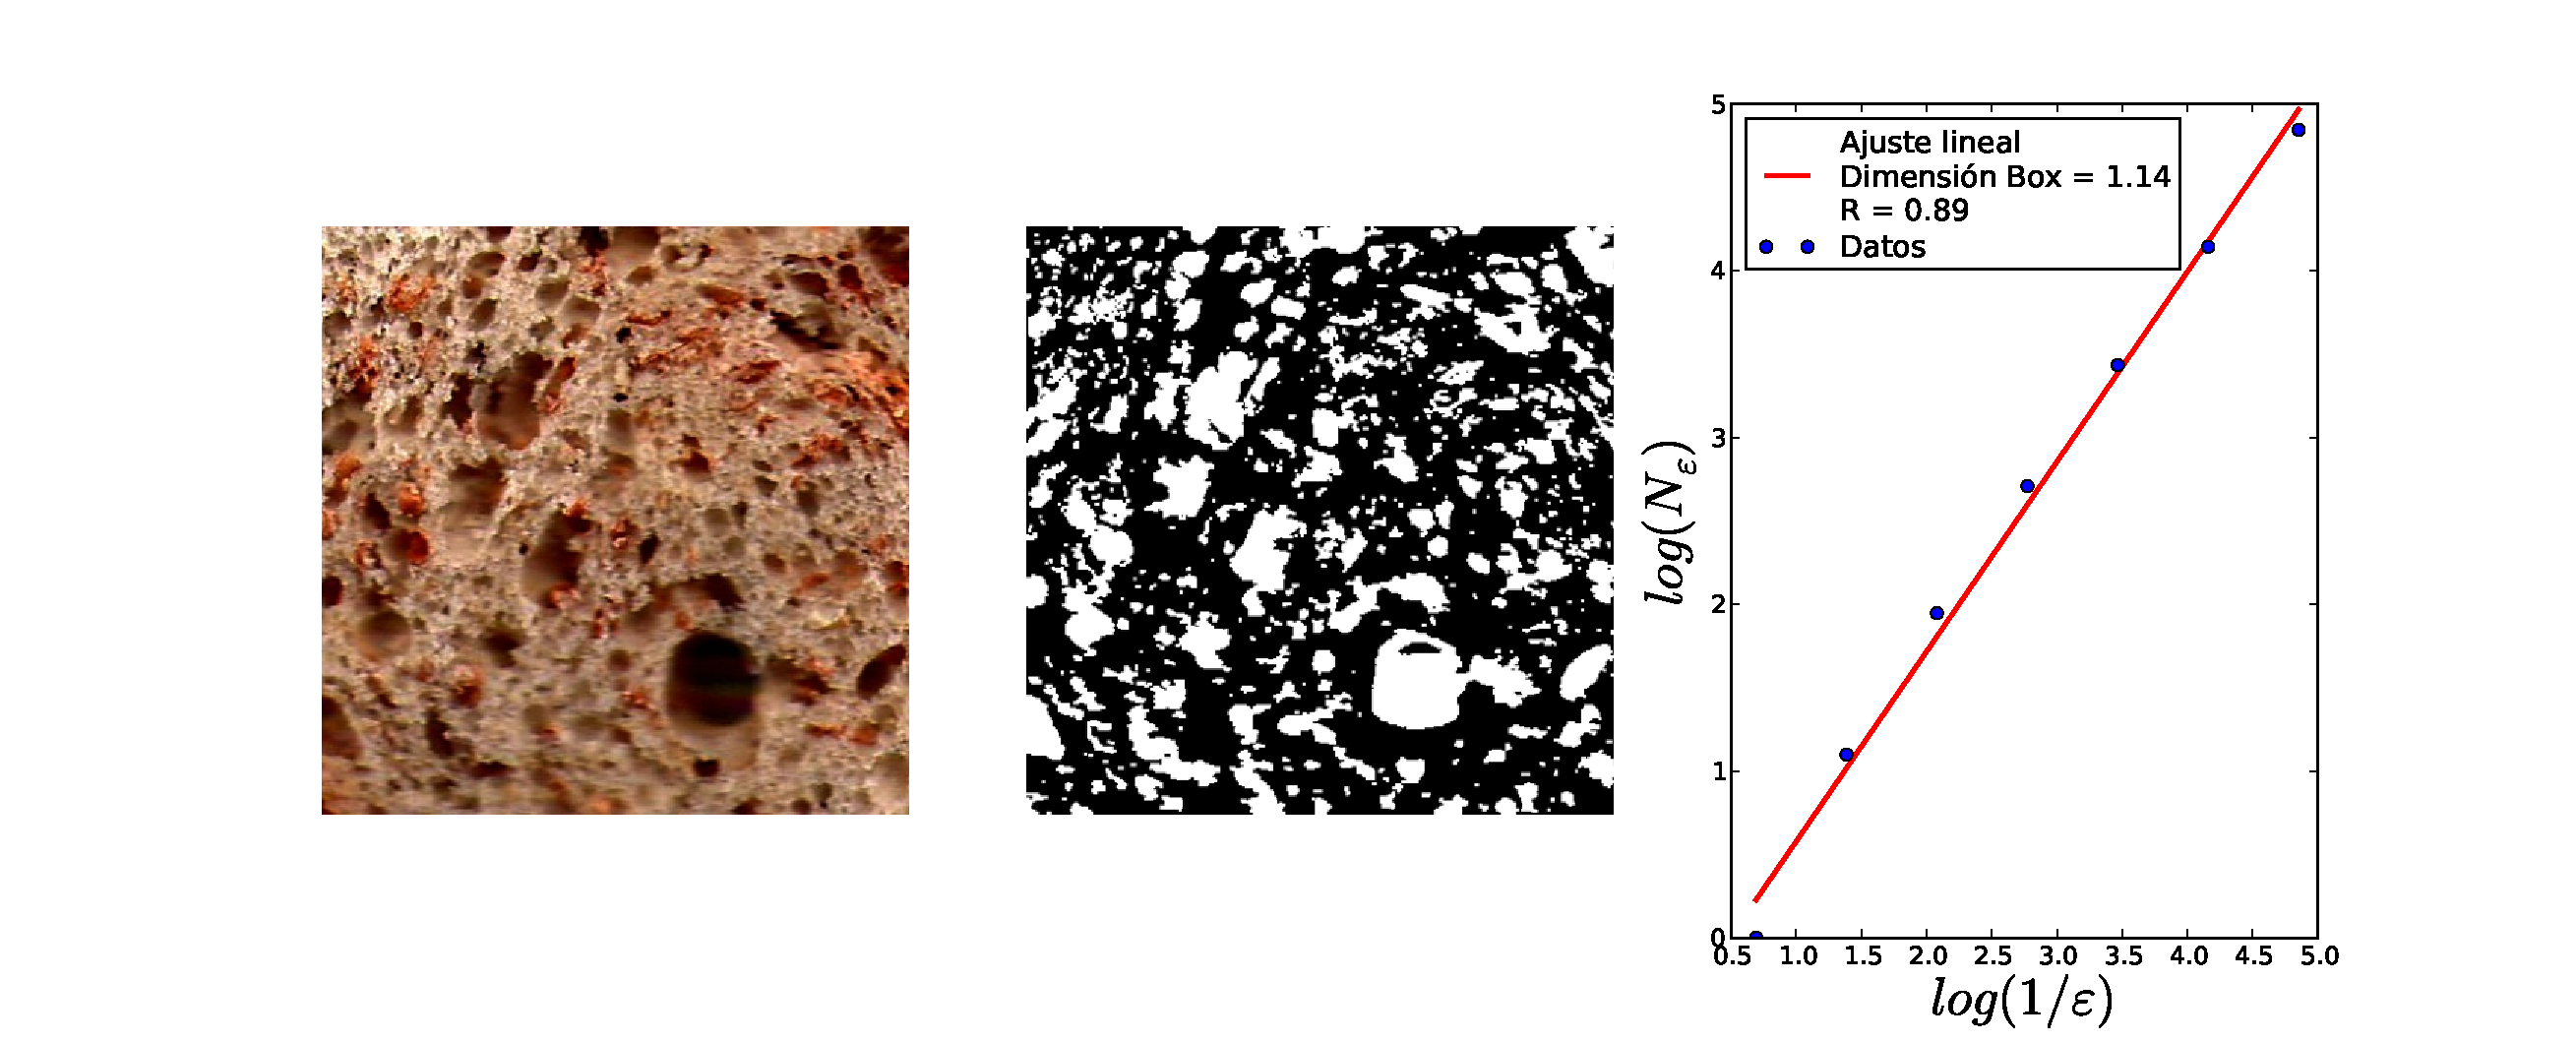
\includegraphics[width=13cm]{dimensionbox}
\caption{Cómputo de la dimensión Box. Una imagen de pan (izquierda) con su binarización (centro) y su dimensión box computada (derecha).}
\label{fig:fitbox}
\end{figure}

\begin{figure}[h!]
\centering
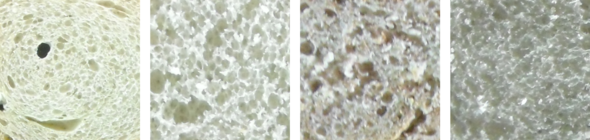
\includegraphics[width=13cm]{pancamara}
\caption{Imágenes de pan tomadas con una cámara digital.}
\label{fig:camera}
\end{figure}

\begin{figure}[h!]
\centering
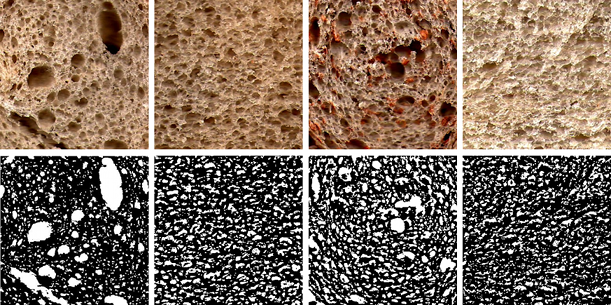
\includegraphics[width=13cm]{binarizaciones}
\caption{Imágenes de distintos tipos de pan tomadas con un escáner. {\em Baguette}, {\em lactal}, {\em salvado} y {\em sandwich} (primera fila) con sus correspondientes binarizaciones utilizando umbralamiento local (segunda fila).}
\label{fig:bread}
\end{figure}

\begin{figure}[h!]
\begin{centering}
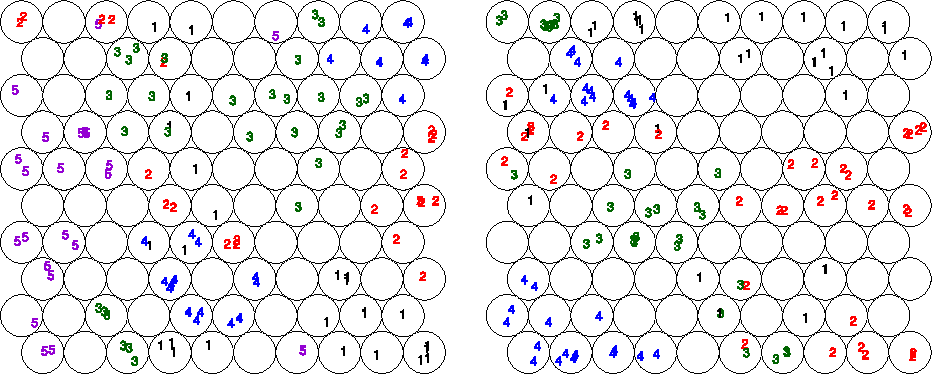
\includegraphics[width=13cm]{SOM}
\caption{Mapas auto-organizados (self-organising maps SOM). SOM de imágenes de panes y no-panes (izquierda) y SOM sólo de tipos de panes (derecha). $1$: {\em baguette}, $2$: {\em lactal}, $3$: {\em salvado}, $4$: {\em sandwich}, $5$: {\em no-pan}.}
\label{fig:somfractal}
\end{centering}
\end{figure}

\begin{figure}[h!]
\centering
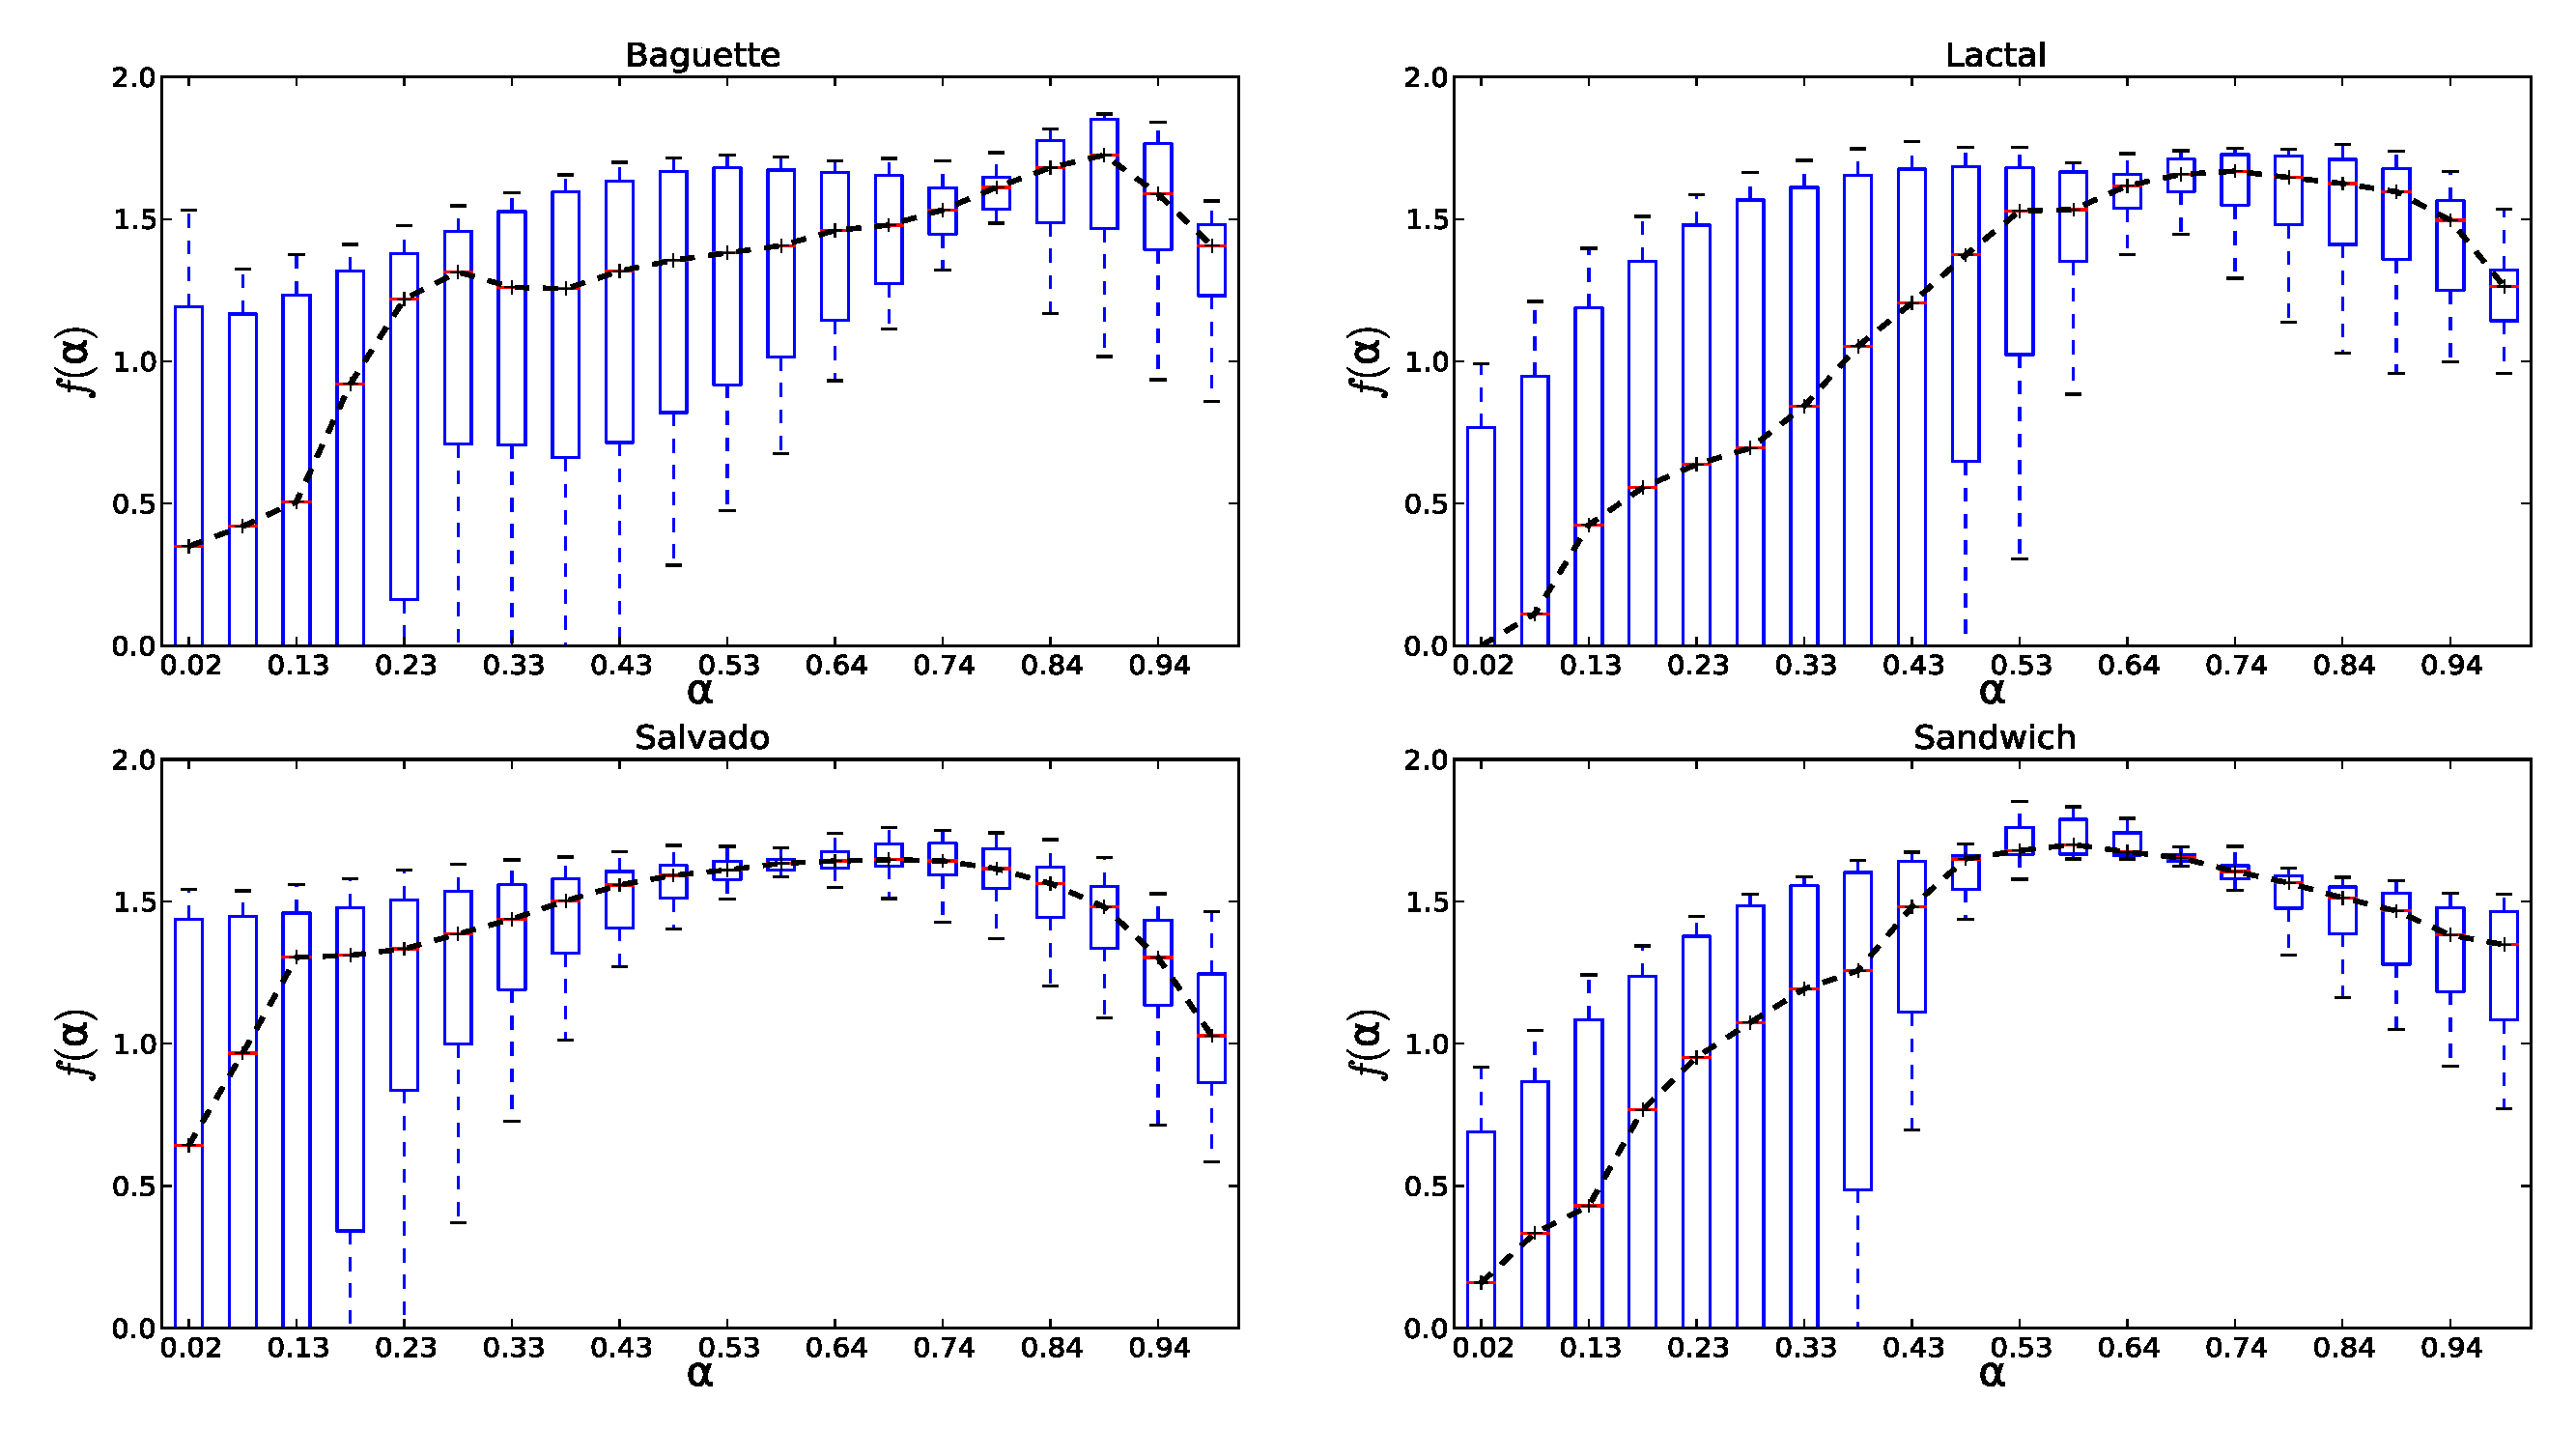
\includegraphics[width=13cm]{boxplots}
\caption{Boxplots de los cuatro tipos de panes. Las medianas de las dimensiones se unen con una línea a trozos. Arriba: {\em baguette} (izquierda), {\em lactal} (derecha), abajo: {\em salvado} (izquierda), {\em sandwich} (derecha).}
\label{fig:boxplotsMFS}
\end{figure}

\begin{figure}[h!]
\centering
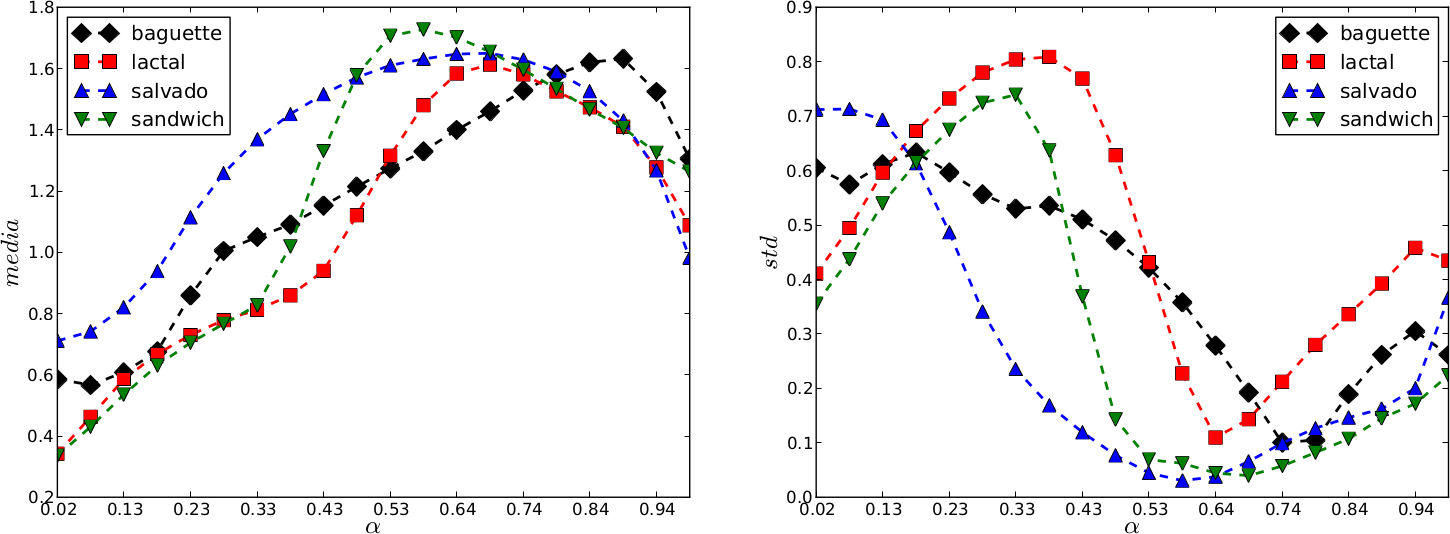
\includegraphics[width=13cm]{panstd}
\caption{MFS promedio y desvíos estándar de las FDs para los cuatro tipos de panes. Izquierda: MFS promedio, derecha: desvíos estándar.}
\label{fig:meansMFS}
\end{figure}


\begin{figure}[h!]
\centering
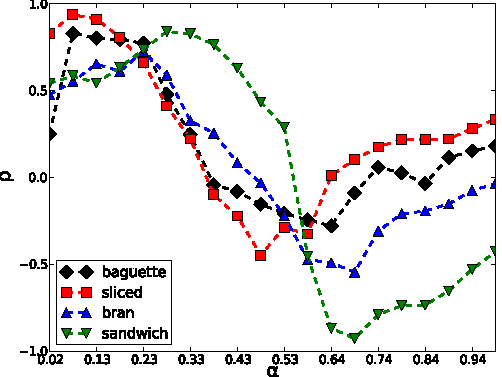
\includegraphics[width=8cm]{VF}
\caption{Coeficiente de correlación Spearman entre las FDs del MFS y la fracción de vacío de las muestras escaneadas.}
\label{fig:corrVF}
\end{figure}

\begin{figure}[h!]
\centering
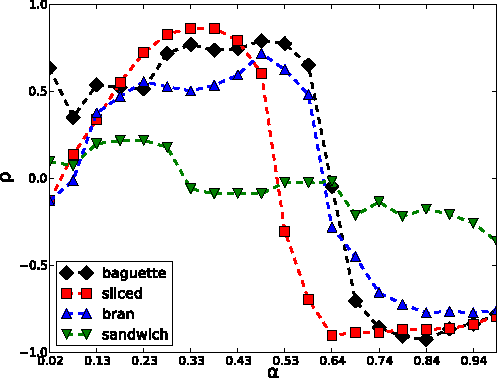
\includegraphics[width=8cm]{MCA}
\caption{Coeficiente de correlación Spearman entre las FDs del MFS y el área media de las burbujas de las muestras escaneadas. (en $[mm^{2}]$).}
\label{fig:corrMCA}
\end{figure}

\begin{figure}[h!]
\centering
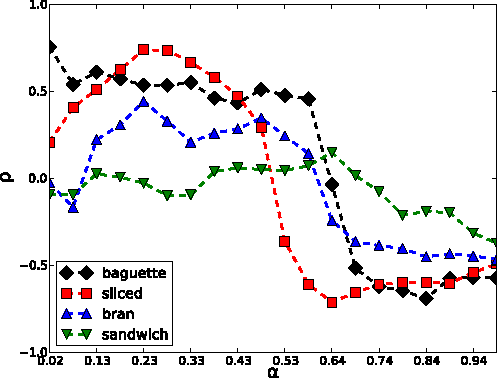
\includegraphics[width=8cm]{stMCA}
\caption{Coeficiente de correlación Spearman entre las FDs del MFS y el desvío estándar del área media de las burbujas de las muestras escaneadas. (en $[mm^{2}]$).}
\label{fig:corrMCAstdev}
\end{figure}




\begin{table}[h!]
\center
% table caption is above the table
\caption{Resultados de la clasificación de migas de pan utilizando diferente número de características para el MFS y diferentes algoritmos de clasificación.}
\label{tab:number}       % Give a unique label
% For LaTeX tables use
\begin{tabular}{lllll}
\hline\noalign{\smallskip}
\#FDs & 10  & 20 & 30 \\
\noalign{\smallskip}\hline\noalign{\smallskip}
SVM & \textbf{96\%} & 94.5\% & 95.5\% \\
RF  & 91.5\% & \textbf{93.5\%} & 93\% \\
NN & 88.5\% & \textbf{90.5\%} & 90\% \\
\noalign{\smallskip}\hline
\end{tabular}
\end{table}


\begin{table}[h!]
\center
% table caption is above the table
\caption{Resultados de la clasificación de migas de pan utilizando diferentes combinaciones del MFS y diferentes algoritmos de clasificación.}
\label{tab:mfs}       % Give a unique label
% For LaTeX tables use
\begin{tabular}{lllll}
\hline\noalign{\smallskip}
Método & MFS & MFS+L & MFS+G & CIELab  \\
\noalign{\smallskip}\hline\noalign{\smallskip}
SVM & 94.5\% & 95.5\% & \textbf{97.5\%} & \textbf{97.5\%} \\
RF  & 93.5\% & \textbf{96\%} & 95\% & \textbf{96\%} \\
NN & 90.5\% & 90\% & 87\% & \textbf{92\%} \\
\noalign{\smallskip}\hline
\#FDs & 20 & 40 & 40 & 60 \\
\hline
\end{tabular}
\end{table}

\begin{table}[h!]
\center
% table caption is above the table
\caption{Resultados de la clasificación de migas de pan para diferentes características del estado del arte y diferentes algoritmos de clasificación.}
\label{tab:other}       % Give a unique label
% For LaTeX tables use
\begin{tabular}{llllll}
\hline\noalign{\smallskip}
Method & Haralick & Lbp & SIFT\\ % & Zernicke
\noalign{\smallskip}\hline\noalign{\smallskip}
SVM & 94\% & 78.5\% & \textbf{96.5\%} \\ % & 55 
RF  & 91\% & 71.5\% & \textbf{92\%} \\ % & 58 
NN & 79\% & 70\% & \textbf{86\%} \\ % & 48.5 
\noalign{\smallskip}\hline
\#FDs & 13 & 36 & 128 \\
\hline
\end{tabular}
\end{table}

\begin{table}[h!]
\center
% table caption is above the table
\caption{Matriz de confusión para los mejores resultados (método CIELab, utilizando el algoritmo de clasificación SVM).}
\label{tab:confusionmatrix}       % Give a unique label
% For LaTeX tables use
\begin{tabular}{llllll}
\hline\noalign{\smallskip}
Clase&{\em baguette} & {\em lactal} & {\em salvado} &{\em sandwich}&{\em no-pan} \\
\noalign{\smallskip}\hline\noalign{\smallskip}
{\em baguette} & 39& 1 &1 &0 &0 \\
{\em lactal} & 0& 38 &0 &0 &0  \\
{\em salvado} & 0& 0 &39 &1 &0  \\
{\em sandwich} & 1& 1 &0 &39 &0  \\
{\em no-pan} & 0& 0 &0 &0 &40  \\
\hline
\end{tabular}
\end{table}


\section{Validación de Imágenes Sintéticas de Pan}

En el capítulo de modelado introdujimos distintos algoritmos para modelar la geometría de la miga del pan.
En esta sección mostraremos que el algoritmo de modelado que atiende al proceso de fabricación del pan puede ser validado utilizando métodos multifractales.

Particularmente, utilizaremos el MFS previamente descripto, pero en otra representación, la cual es la más adecuada para los propósitos de este capítulo.
Esta forma de computar el MFS es ampliamente utilizada en análisis de texturas en visión por computadoras y en análisis de patrones.
A diferencia de los fractales\cite{Gonzales2008}, la teoría multifractal ha sido utilizada para describir características de imágenes, pero no en caracterización de panes.

Existen dos clases principales de espectro multifractal: dimensiones generalizadas ($D_{q}$) y exponentes de Lipschitz-H\"older ($f(\alpha)$). 
La última representación es útil para realizar clasificación, como fue mostrado.

Las dimensiones multifractales generalizadas pueden ser computadas de muchas maneras, de las cuales el método Sandbox \cite{Tel1989} calcula el valor medio de muchas muestras aleatoriamente distribuidas, sobre puntos pertenecientes a la estructura \cite{Debartolo2004}. 

La dimensión generalizada de orden $q$ con el método Sandbox se define como:

 \begin{align*}
D_{q\ne 1}^{sb} &= \frac{1}{q-1} \lim_{R \rightarrow 0}{
\frac{ln   { \left\langle  (M(R)/M_{0})^{q-1} \right\rangle   }}
{ln {(R/L)}       }},\\
D_{q=1}^{sb} &= \lim_{R \rightarrow 0}{
\frac{ \left\langle ln   { (M(R)/M_{0})  }  \right\rangle}
{ln {(R/L)}       }},
\end{align*}
%
donde $M_{0}$ es la cantidad de píxeles blancos en la imagen binarizada y $M(R)$ es el número de puntos que pertenecen a la estructura en un círculo de radio $R$ centrado en un punto de la misma.

Cuando $q\ne1$, computamos el límite como la pendiente del ajuste lineal de los valores $ln(R/L)$ vs. $ ln  \left\langle  { (M(R)/M_{0})^{q-1} }  \right\rangle$, para $R$ en $[R_{min}, R_{max}]$, donde $ \left\langle \cdot  \right\rangle$ denota el valor medio sobre los puntos muestreados.
Se procede similarmente para $q=1$. 
Computando el valor para diferentes $q \in [Q_{\min},Q_{\max}]$  se obtiene el espectro sandbox.

Esta clase de análissi es reportada como la más adecuada para análisis de características texturales y geométricas \cite{Gonzales2008}, por lo que lo utilizamos sobre $10$ imágenes binarizadas a partir de muestras escaneadas de migas de pan del tipo {\em baguette}, y $10$ imágenes sintéticas producidas con nuestro método luego del paso de cocción, obteniendo $20$ vectores de características.
Luego separamos cada clase y computamos boxplots para las dos clases.
Las migas de pan fueron manualmente segmentadas para prevenir errores de segmentación automática, similarmente a como fue hecho en \cite{Bosch2011}.

El modelo tiene $5$ parámetros:

\begin{align*}
N &= \frac{k}{r^{d}},\\ r &= r_{min}+paso*j, j \in [0,\frac{r_{max}}{paso}],
\end{align*}
$k,d,r_{min},r_{max}$ y $step$ que controlan la generación de burbujas en el paso de leudado.
Para computar el espectro sandbox de cada imagen, utilizamos $1000$ puntos aleatorios distintos para asegurar estabilidad en el espectro resultante.

Los parámetros definen un espacio de búsqueda, en el cual implementamos una búsqueda semi automática definiendo una métrica de error:
\begin{equation*}
Error = \displaystyle \sum abs(medianas_{real}-medianas_{sint\acute{e}tico}),
\end{equation*}
y encontramos el menor error en la siguiente configuración de parámetros,
\begin{align*}
k &= 0.07 \frac{N^{3}}{20} ,\\
d &=2.78,\\
r_{min} &=2,\\
r_{max} &=20.\\
paso &=1,
\end{align*}

donde $N$ es la cantidad de voxels en cada dimensión durante el leudado (elegimos $N = 512$). 
El error acumulado en medianas es de $\sim 0.21$, lo cual significa un error promedio de $0.21/21 \sim 0.01$ en cada dimensión.
La Fig.~\ref{bestboxplot} muestra boxplots de panes reales y sintéticos con las medianas de cada dimensión unidas por líneas de puntos.
Cuando $q < 0$ las dimensiones presentan una dispersión mayor, ya que el método aproxima esas dimensiones de un modo menos preciso.
La Figura muestra espectros casi idénticos para panes reales y sintéticos.
Las Fig.~\ref{realbin} y Fig.~\ref{best} muestran un ejemplo de binarizaciones de un pan real y sintético utilizando estos parámetros de genración.


\begin{figure}[!ht]
\includegraphics[width=9cm]{figures/bestboxplot}
\caption{Mejores parámetros para el tipo de pan {\em baguette}. El error total en medianas es de $\sim 0.21$.}
\label{bestboxplot}
\end{figure}

\begin{figure}[!ht]
\begin{center}
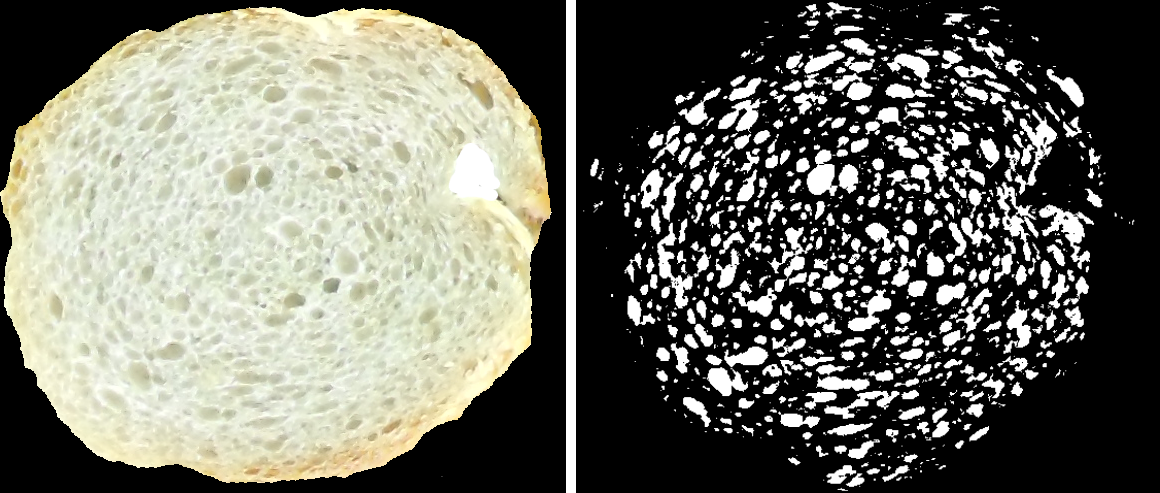
\includegraphics[width=13cm]{figures/realbin}
\caption{ Pan {\em baguette} real y ejemplo de binarización.}
\label{realbin}
\end{center}
\end{figure}

\begin{figure}[!ht]
\begin{center}
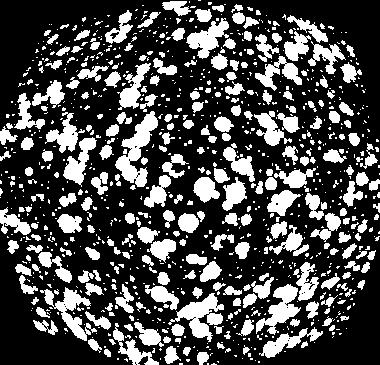
\includegraphics[width=6cm]{figures/best}
\caption{Resultado sintético mostrando características multifractales similares a imágenes reales del tipo de pan {\em baguette}.}
\label{best}
\end{center}
\end{figure}

Similarmente, encontramos parámetros para un tipo de pan casero utilizando la misma búsqueda:

\begin{align*}
k &= 0.69 \frac{N^{3}}{20} ,\\
d &=5.6,\\
r_{min} &=1,\\
r_{max} &=24.\\
paso &=1,
\end{align*}

La Fig.~\ref{bestboxplot2} muestra boxplots de panes reales y sintéticos de este tipo casero.
La Fig.~\ref{realbin2} y  Fig.~\ref{best2} muestran un ejemplo de binarizaciones de estas imágenes. 


\begin{figure}[!ht]
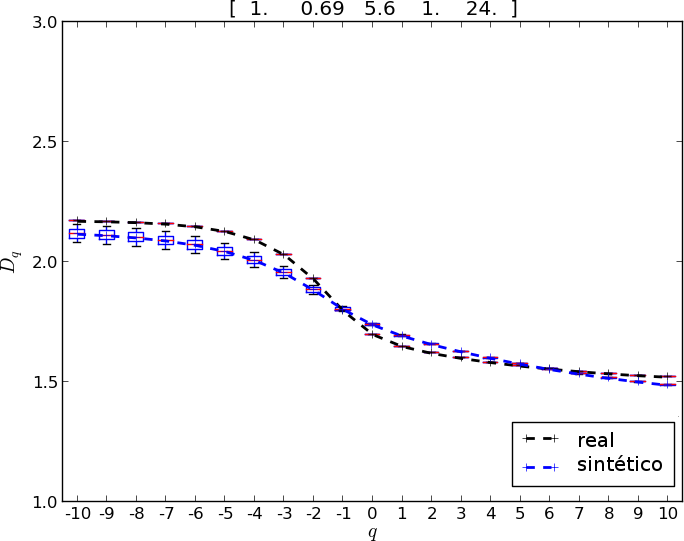
\includegraphics[width=9cm]{figures/bestboxplot2}
\caption{Mejores parámetros para un tipo casero de pan. El error total en medianas es de $\sim 0.88$.}
\label{bestboxplot2}
\end{figure}

\begin{figure}[!ht]
\begin{center}
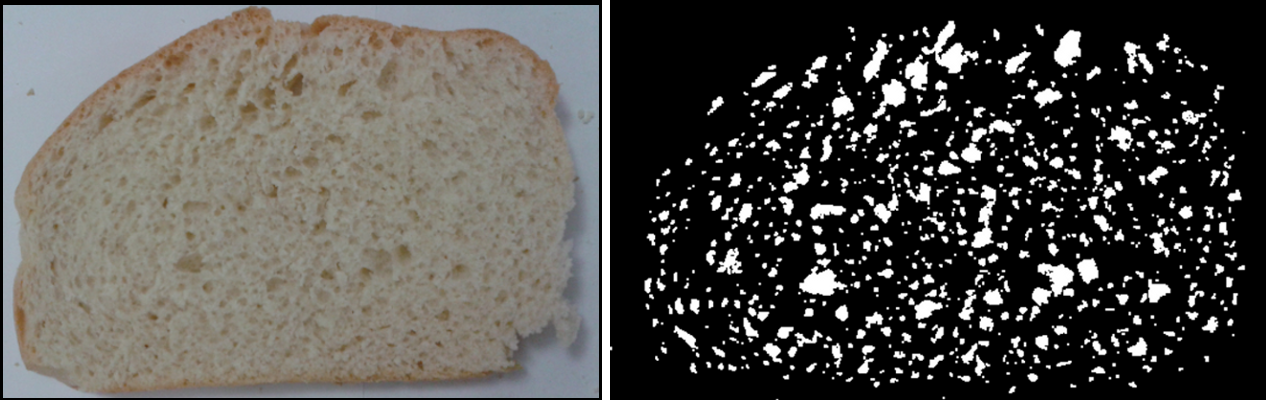
\includegraphics[width=13cm]{figures/realbin2}
\caption{ Pan casero real y ejemplo de binarización.}
\label{realbin2}
\end{center}
\end{figure}

\begin{figure}[!ht]
\begin{center}
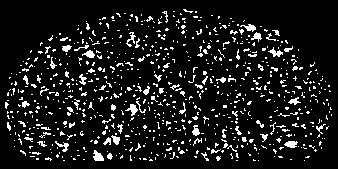
\includegraphics[width=8cm]{figures/best2}
\caption{Ejemplo de pan sintético con características similares a imágenes de un pan casero.}
\label{best2}
\end{center}
\end{figure}


%We apply the sandbox multifractal method to study the geometry we obtained after the deformation step. This method is best suited for geometrical measurements than other multifractal approaches.

%We apply the sandbox method to $10$ binarised real bread crumb images of the {\em baguette} bread type that we captured with a digital scanner and $10$ syhthetic images produced using our pipeline, after the deformation step, obtaining $20$ feature vectors. Then we separate each class and we compute boxplots for the two classes. We manually segmented real bread crumbs to prevent automatic segmentation errors as in \cite{Bosch2011}. The model has $5$ parameters:


%\begin{align}
%N_{spheres} &= \frac{k}{r^{d}},\\ r &= v_{min}+step*j, j \in [0,\frac{v_{max}}{step}]
%\end{align}
%$k,d,v_{min},v_{max}$ and $step$ that controls bubble's generation in the proving stage. %To compute the sandbox spectrum of each image, we used $5000$ different random points to ensure stability in the resulting spectrum.

%We implemented an automated search in parameter space and we found that the following parameters produce the lowest error:

%\begin{align*}
%k &= 0.07 \frac{N_{x}\times N_{y}\times N_{z}}{20} ,\\
%d &=2.78,\\
%v_{min} &=2,\\
%v_{max} &=20.\\
%step &=1,
%\end{align*}
%\noindent where $N_{x}$, $N_{y}$ and $N_{z}$ are the proving volume dimensions in each spatial coordinate (we chose $(N_{x},N_{y},N_{z}) = (760,760,100)$). The accumulated error in medians is $\sim 0.21$ meaning a mean error of $0.21/21 \sim 0.01$  in each dimension. We compute this error as:

%\begin{equation}
%Error = \displaystyle \sum abs(means_{real}-means_{synthetic}).
%\end{equation}
%Fig.~\ref{bestboxplot} shows boxplots of real and synthetic breads with the medians for each dimension joined by dashed lines. When $q < 0$ dimensions have a higher dispersion, since the method approximates these dimensions less accurately. The figure shows almost identical spectra for real and synthetic breads.  Fig.~\ref{realbin} and  Fig.~\ref{bestwarp} show an example of real and synthetic binarisations for these parameters.

%\begin{figure}[!ht]
%\includegraphics[scale=0.5]{bestboxplot.png}
%\caption{Best fitting parameters. The total error in medians is $\sim 0.21$.}
%\label{bestboxplot}
%\end{figure}

%\begin{figure}[!ht]
%\begin{center}
%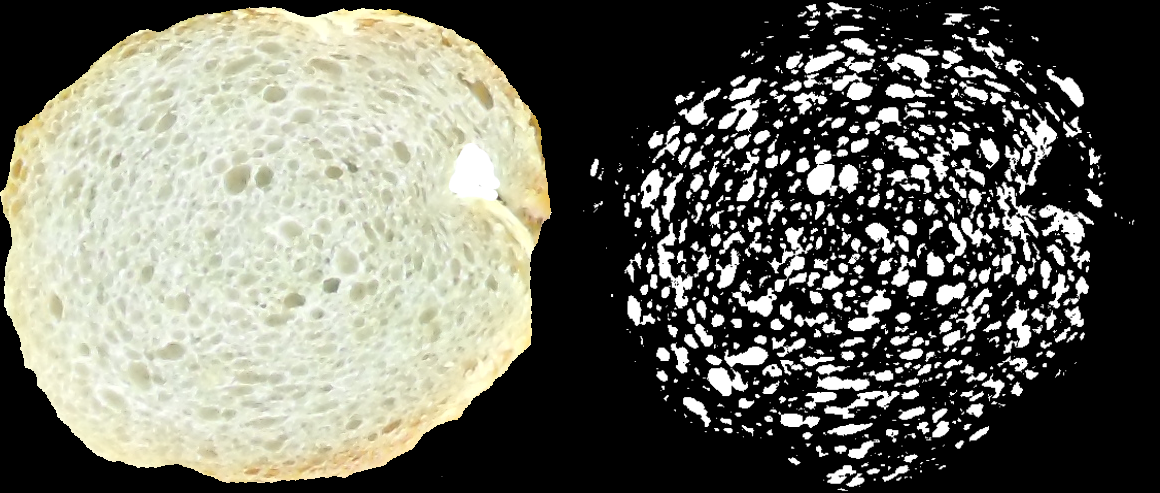
\includegraphics[scale=0.2]{realbin.png}
%\caption{ Real bread and binarisation example.}
%\label{realbin}
%\end{center}
%\end{figure}

%\begin{figure}[!ht]
%\begin{center}
%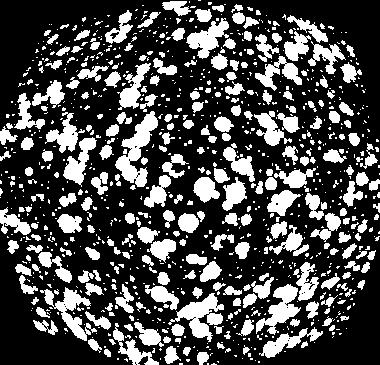
\includegraphics[scale=0.4]{bestwarp.png}
%\caption{Model distribution example showing similar multifractal features to real breads .}
%\label{bestwarp}
%\end{center}
%\end{figure}


%Automated searchs in parameter space may be useful to automatically match other bread types and materials.

%\section{Resultados}

%\section{Validación utilizando técnicas de Aprendizaje Profundo}

\section{Discusión y Conclusiones}

En este capítulo mostramos que los métodos fractales y sobre todo, multifractales, permiten capturar características útiles de panes, las cuales sirven para caracterizarlos y clasificarlos.
Además, la información capturada es lo suficientemente descriptiva como para definir parámetros de entrada a un algoritmo que genera versiones sintéticas de los mismos, las cuales fueron también validadas.


La apariencia visual de diferentes tipos de panes puede ser caracterizada exitosamente computando dimensiones multifractales de sus imágenes digitales.
Las DFs obtenidas por el método MFS cuyo $\alpha \in [0,0.23]$ proveen una buena medida de la porosidad de la miga del pan, ya que mientras más alta es la DF, más alta es la porosidad.
Además, las DFs cuyo $\alpha \in [0.79,1]$ permiten caracterizar la granularidad y la heterogeneidad en la distribución de sus burbujas.
El MFS contiene datos útiles para caracterizar las tres medidas, combinando la información en un único vector de características.

La utilización de características multifractales en la clasificación de dichas imágenes mostró además una excelente performance.
El MFS demostró ser lo suficientemente preciso para realizar una clasificación de distintos tipos de panes y de separar panes de otros objetos.
Los resultados superan otras características del estado del arte utilizadas en la literatura de visión por computador.
La información presente en los canales $L$, $a$ y $b$ del MFS de las imágenes transformadas al espacio de color CIELab obtuvieron los mejores resultados en la clasificación.
Este resultado parece ser consecuencia del comportamiento del espacio mencionado cuando existe más de un dispositivo de captura.
Se mostró además que el MFS es sensible a cambios en la iluminación durante la adquisición de las imágenes.

Por otro lado, el método multifractal sanbox permite aproximar la geometría de cualquier miga de pan, extrayendo parámetros para simular de manera precisa un tipo dado.
Las distribuciones de burbujas de nuestro modelo pueden adecuarse de manera estadística con algún tipo de pan deseado, gracias al análisis multifractal sandbox.
El método produce imágenes con características multifractales similares a panes reales.
Para comprobar esta afirmación, se realizaron comprobaciones con dos tipos de pan diferentes, {\em baguette} y un tipo de pan casero.
El espectro multifractal del pan casero resultó más dificultoso de sintetizar (es decir, los errores fueron mayores que aquellos del tipo {\em baguette}), pero a pesar de esto, las imágenes obtenidas resultan más que adecuadas para emular el tipo de pan deseado en computación gráfica.

El espectro multifractal mostró mayor dispersión en las dimensiones negativas ($q < 0$), 
lo cual significa que debido al límite de resolución en las imágenes, la distribución estadística es más difícil de capturar en escalas más pequeñas.



%A more detailed link between bread crumb physical features (coarseness, porosity) and multifractal features may be useful for designing better procedural models \cite{Baravalle2012}.
%Multifractal image analysis was used to validate the model.
%The statistical similarity between $2D$ cuts in our results and of real-word bread slices suggests that it may be suitable for applications in $3D$ engines, serious games \cite{Susi2007} and photorealistic rendering. 

%citar imfractal


